\chapter{ZigBee}

ZigBee is widely used in various fields from home automation to Mars exploration; it is considered the ``cousin'' of Bluetooth: they are standardized by the same company and can coexist.

\begin{paracol}{2}

   \colfill
   Aside from the application layer, ZigBee defines also a \textit{Network Layer} which perfectly matches and maps to the underlying MAC and Physical Layers, standardized by \texttt{IEEE 802.15.4};
   ZigBee is built on top of such IEEE standard.
   \colfill

   \switchcolumn
   
   \begin{figure}[htbp]
      \centering
      \includegraphics{images/zigbee_layers.png}
      \caption{ZigBee layers}
      \label{fig:zigbee_layers}
   \end{figure}
\end{paracol}

\labelitemize{\textit{Key Features}}{
   \begin{itemize}
      \item Specification of the physical and MAC layers for low-rate Wireless Personal Area Networks (PAN)
      \item Infrastructure-less
      \item Short range\footnote{250m outdoors in ideal conditions}
      \item Support for star and peer-to-peer topologies
      \item Can coexist with IEEE 802.11 and IEEE 802.15.1 (Bluetooth)
      \item Works on licence-free frequency bands
   \end{itemize}
}

\section{Architecture}

\begin{paracol}{2}
   
   
   APS provides \textit{transport} services to the ZDO and the Objects in the Application Framework (APOs). It is some kind of Transport layer, similar to TCP but not the same.
   
   APOs are the business logic of the business device, implemented by the user, and in a single device there may be instantiated up to APOs.
   We may say that for each APO provides a ``functionality''.
   
   The ZDO is an applicative object that defines and maintaines the device behaviour in a ZigBee network.
   \note{An example of this behaviour, is replying to a device discovery message. Such reply is handled by the ZDO}
   The ZDO is provided by the third parties which are giving you the ZigBee stack.
   Manufacturers which produce devices compliant with ZigBee, sell them with a ZigBee stack already implemented, allowing for the buyer ---e.g. a company which develops ZigBee solutions--- to simply implement the ``functionalities'' (i.e. APOs) they want.
   \switchcolumn

   \begin{figure}[htbp]
      \centering
      \includegraphics{images/zigbee_architecture.png}
      \caption{Zigbee architecture layers}
      \label{fig:zigbee_architecture}
   \end{figure}
\end{paracol}

\section{Primitives}
\begin{figure}[htbp]
   \centering
   \includegraphics{images/zigbee_primitives.png}\\
   \includegraphics{images/zigbee_primitives2.png}
   \caption{Mapping between zigbee primitives}
   \label{fig:zigbee_primitives}
\end{figure}

\labelitemize{Primitives}{
   \begin{enumerate}
      \item \texttt{Request}\\
      It is invoked by the upper layer to request for a specific service
      \item \texttt{Indication}\\
      Is a sort of \textit{``upcall''}, generated by the lower layer and is directed to the upper layer to notify the occurrence of an event related to a specific service
      \item \texttt{Response}\\
      It is invoked by the upper layer to complete a procedure previously initiated by an indication primitive
      \item \texttt{Confirm}\\
      It is generated by the lower layer and is directed to the upper layer to convey the results of one or more associated previous service requests.
   \end{enumerate}
}

\section{Network Layer}

The ZigBee network layer provides services for:
\begin{enumerate}
   \item Data transmission (both unicast and multicast)
   \item Network initialization
   \item Devices addressing
   \item Routes management \& routing
   \item Management of joins/leaves of devices
\end{enumerate}

In a ZigBee network there are three kinds of devices:
\begin{enumerate}
   \item \textbf{The Network coordinator}
      
   A FFD\footnote{Full functional Device} that creates and manages the entire network
   \item \textbf{Routers}
      
   A FFD with routing capabilities
   \item \textbf{End-devices}
   
   Correspond to a RFD\footnote{Reduced functional device} or to a FFD acting as simple devices
\end{enumerate}

\begin{figure}[htbp]
   \centering
   \includegraphics{images/zigbee_networktopologies.png}
   \caption{ZigBee Network topologies outline}
   \label{fig:zigbee_networktopologies}
   The superframe mentioned above, is a feature used to obtain energy efficiency in ZigBee networks, but we will discuss it later on.
\end{figure}

\subsection{Network formation and joining}
Before communicating on a network, a ZigBee device must either:
\begin{itemize}
   \item Form a new network $\longrightarrow$ \textit{ZigBee Coordinator}
   \item Join an existing network $\longrightarrow$ \textit{ZigBee router} or \textit{end-device}
\end{itemize}
\note{The role of the device is chosen at compile-time}

\subsubsection{Formation}
\begin{paracol}{2}
   \colfill
   \textbf{Network Formation} is performed by a coordinator, which uses the MAC layer services to (\texttt{SCAN.request}) look for a channel that does not conflict with other existing networks, and then selects a PAN identifier which is not already in use by other PANs.
   \colfill
   \switchcolumn
   \begin{figure}[htbp]
      \centering
      \includegraphics{images/zigbee_netformation.png}
      \caption{Network formation messages}
      \label{fig:zigbee_netformation}
   \end{figure}
\end{paracol}

\subsubsection{Joining}
\begin{paracol}{2}
   \colfill
   Joining may happen in two ways, the first is to \ul{join through \textbf{association}}: 
   initiated by a device wishing to join an existing network.
   
   Alternatively a device may \ul{perform a 
\textbf{Direct join}}:
   requested by a router or by the coordinator to request a device to join its PAN.
   \colfill
   \switchcolumn
   \begin{figure}[htbp]
      \centering
      \includegraphics{images/zigbee_netjoining.png}
      \caption{Network joining messages}
      \label{fig:zigbee_netjoining}
   \end{figure}
\end{paracol}

\section{Application Layer}

Up to 240 APOs, each corresponding to an application \textbf{Endpoint}, with the Endpoint 0 reserved for the ZDO\footnote{We could say that the ZDO is an ``application object'', which would be true, but tailored to specific needs}.
\ul{Each APO in the network is uniquely identified by its endpoint address and the network address} of the hosting device.

\subsection{APS - Application Support Sublayer}
The APS frame uses the concepts of \textbf{endpoints}, \textbf{cluster
ID}s, \textbf{profile ID}s and \textbf{device ID}s.\\
It provides:
\begin{itemize}
   \item Data service (a light transport layer)
   \begin{itemize}
      \item Filtering out packets (non registered endpoints, profiles that do
      not match)
      \item Generating end-to-end acknowledgments
   \end{itemize}
   \item Management:
   \begin{itemize}
      \item Local binding table
      \item Local groups table
      \item Local address map
   \end{itemize}
\end{itemize}

\subsubsection{Concepts and related IDs}

\begin{paracol}{2}
   A \textbf{cluster} may be, in the simplest case, a \textit{message}. But this is not necessarily the case.\\
   Informally, a cluster provides access to a service (a functionality) of an application object;
   \ul{Defines both \textit{commands}}, which cause actions on a device, \ul{and \textit{attributes}}, showing the state of a device in a given cluster.\\
   \note{\ul{Every cluster has a 16 bit identifier}, which according to prof. Chessa is \textbf{not} sufficient.}
   
   Note that clusters are not related to the physical world interaction, because they must allow reuse.\\
   Each cluster finds a possibly different meaning in each \textbf{application profile}. There is a mapping which defines such meanings mappings.
   \note{Using this schema, 16 bits become sufficient.}
   
   An \textbf{application profile} is the specification of the
   behaviour of a class of applications possibly operating
   on several ZigBee devices.
   Each profile is paired with a 16 bit identifier.
   \note{Every message sent (or received) is tagged with a profile ID.
   Different application profiles may co-exist in a single
   ZigBee network.}
   \switchcolumn

   \begin{figure}[htbp]
      \centering
      \includegraphics{images/zigbee_generalclusters.png}\\
      \includegraphics{images/zigbee_appprofiles.png}
      \caption{ZigBee General Domain clusters and common Profile IDs}
      \label{fig:zigbee_generalclusters}
   \end{figure}
\end{paracol}

\begin{paracol}{2}
   ZigBee \textbf{Device ID}s range from \texttt{0x0000} to \texttt{0xFFFF}, and have two purposes:
   \begin{enumerate}
      \item To allow human-readable displays (e.g., an icon related to a device)
      \item Allows ZigBee tools to be effective also for humans
      \begin{enumerate}
         \item a device may implement the on/off cluster, but you don’t know whether it is a bulb or a oven \dots you only know you can turn it on or off.
         \item The device ID tells you what it is, but it does not tell you how to communicate with it, which is given by the IDs of the clusters it implements!
      \end{enumerate}
   \end{enumerate}
   \note{ZigBee discovers services in a network based on profile IDs
   and cluster IDs, but \textbf{not} on device IDs}

   \switchcolumn

   \begin{figure}[htbp]
      \centering
      \includegraphics{images/zigbee_deviceIDs.png}
      \caption{Device IDs from the \textit{Home Automation} profiles}
      \label{fig:zigbee_deviceIDs}
   \end{figure}
\end{paracol}

\subsubsection{Back to APS Services}
APS Provides:
\begin{itemize}
   \item Data service to both the APOs and the ZDO.
   \item Binding service to the ZDO
   \item Group management services
\end{itemize}

The APS data service enables the exchange of messages between two or more devices within the network.
\begin{itemize}
   \item The data service is defined in terms of the primitives:
   \item Request (\texttt{send}),
   \item Confirm (returns \texttt{status} of transmission) and
   \item Indication (\texttt{receive}).
\end{itemize}

APS provides also a \textbf{message reliability service}, which simply sends multiple times a message until an ACK is received (if it was needed in the first place).

The \textbf{group management} provides services to build and maintain groups of APOs, enabling multicast, with each group being identified by a 16-bits address.



\note{MAC addresses in ZigBee contexts are meant to be permanent, even if in recent years FFDs provide functionalities to randomly generate MAC addresses in order to enforce privacy.
This in general is not performed on low-end RFD devices.}

\section{Binding}
Addresses are indirect, allowing to implicitly specify the destination of messages, which are no longer routed based on a pair $\langle destination endpoint, destination network address \rangle$ (\textit{direct addressing}), but binding tables and address maps are used instead.

This is one of the key functions of the ZigBee Transport Layer, and is performed by the \textit{APS}.

\subsection{APS - Address Map}
The APS layer contains the address map table, which associates the 16 bit NWK address with the 64 bit IEEE
MAC address.\\
Zigbee end devices (ZED) may change their 16 bit NWK
address (e.g. they leave and join again). In that case an
announcement is sent on the network and every node
updates its internal tables to preserve the bindings.
\begin{figure}[htbp]
   \centering
   \includegraphics{images/zigbee_addressmap.png}
   \caption{Address Map}
   \label{fig:zigbee_addressmap}
\end{figure}

\subsection{APS - Binding}
We assume that typically the binding is performed by an admin who is ---physically--- deploying network nodes. 
\labelitemize{\textit{Primitives}}{
   \begin{itemize}
      \item \texttt{BIND.request}\\
      Creates a new entry in the local binding table taking as input $\langle \textit{source address, source endpoint, cluster identifier, destination address, destination endpoint}\rangle$
      \item \texttt{UNBIND.request}\\
      deletes an entry from the local
      binding table.
   \end{itemize}
}
The binding table associates sources and destinations based on MAC addresses, and is stored in the APS of the ZigBee coordinator (and/or of the routers); it gets updated on explicit request of the ZDO in the routers or in the
coordinator, and is usually initialised at the network deployment.
In general, it is \textit{static}.

\begin{figure}[htbp]
   \centering
   \includegraphics{images/zigbee_bindingtable.png}
   \caption{Binding table}
   \label{fig:zigbee_bindingtable}
\end{figure}

Indirect addressing is implemented exploiting the binding table and the address map:
\begin{itemize}
   \item 
   matches \textit{source address} $\langle \textit{network addr, endpoint addr}\rangle$ and the
   \textit{cluster identifier} into the pair:
   $\langle \textit{destination endpoint, destination network addr}\rangle$
\end{itemize}

\section{ZDO - ZigBee Device Object}
ZDO is a special application attached to endpoint 0 and  implements ZigBee End Devices, ZigBee Routers and
ZigBee Coordinators.

It is specified by a special profile, the ZigBee Device
Profile, which describes the clusters that must be supported by any ZigBee device; it defines also how the ZDO implements the services of discovery and binding and how it manages network and security.

\labelitemize{
   \textit{ZDO services}
}{
   \begin{itemize}
      \item Device and service discovery
      \item Binding management
      \item Network management
      \item Node management
   \end{itemize}
}
\subsection{Device and service discovery}
The ZigBee Device Profile (ZDP) specifies the device and
service discovery mechanisms.
\textbf{Device discovery} allows a device to obtain the (network or MAC) address of other devices in the network:
\begin{itemize}
   \item \textbf{Unicast} $\longrightarrow$ directed to an individual device
   \item \textbf{Broadcast} $\longrightarrow$ hierarchical implementation based on a tree and subtrees topology: a router returns to its parent its address and the address of all the
   end devices associated to itself and then the coordinator returns the address of its associated devices
\end{itemize}

\textbf{Service discovery} exploits queries based on profiles ID, cluster IDs, addresses, or device
descriptors. Again may either be unicast or broadcast.
\begin{itemize}
   \item \textbf{Unicast} $\longrightarrow$ if directed to a single end device then the coordinator or the router to which it is connected respond on its behalf
   \item \textbf{broadcast}$\longrightarrow$
   The coordinator responds to service discovery queries returning lists of endpoint addresses matching with the query;
   It exploits a hierarchical implementation: each router collects information from
   its associated devices and forwards it to its parent
\end{itemize}
   
\subsection{Binding management}
The ZDO processes the binding requests received from local or remote EP To \textit{add} or \textit{delete} entries in the APS binding table.

\subsection{Network and Node Management}
\begin{itemize}
   \item \textbf{Network management}
   \begin{itemize}
      \item Implements the protocols of the coordinator, a router or an
      end device according to the configuration settings established
      either via a programmed application or at installation.
   \end{itemize}
   \item \textbf{Node management}
   \begin{itemize}
      \item The ZDO serves incoming requests aimed at performing
      network discovery, retrieving the routing and binding tables of
      the device and managing joins/leaves of nodes to the
      network.
   \end{itemize}
\end{itemize}

\section{ZigBee Cluster Library}
ZCL is a repository for cluster functionalities, a “working library” with regular updates and new functionalities.
ZigBee developers are expected to use the ZCL to find relevant cluster functionalities to use for their applications, in order to 
\begin{itemize}
   \item Avoid re-inventing the wheel
   \item Support interoperability
   \item Facilitate maintainability
\end{itemize}

A cluster is a collection of commands and attributes, which define an
interface to a specific functionality of a device.
Clusters refer to functional domains within the respective profile.\\
The ZCL forsees a Client-Server model.
\begin{itemize}
   \item The device that \textit{stores} the attributes is the \textit{server} of the cluster
   \item The device that \textit{manipulates} the attributes is the \textit{client} of the cluster
\end{itemize}
\begin{figure}[htbp]
   \centering
   \includegraphics{images/zigbee_functionaldomains.png}
   \caption{Functional domains}
   \label{fig:zigbee_functionaldomains}
\end{figure}

TODO integrate some slides

ZCL is built to allow combining simpler clusters into more complex ones, providing a hierarchical approach to define device functionalities.

\begin{figure}[htbp]
   \centering
   \includegraphics{images/zigbee_zclcombining.png}
   \caption{ZCL Hierarchical approach}
   \label{fig:zigbee_zclcombining}
\end{figure}

\begin{figure}[htbp]
   \centering
   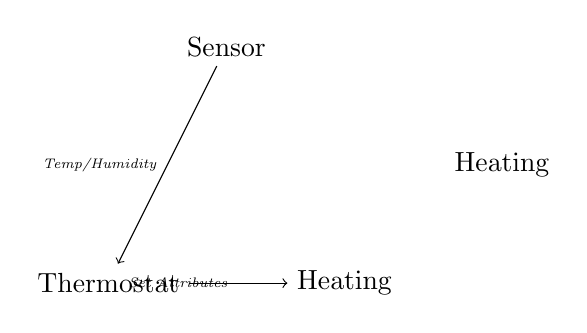
\begin{tikzpicture}
      \node[draw=white,align=left] (S) at (1.5,3) {Sensor};
      \node[draw=white,align=left] (T) at (0,0) {Thermostat};
      \node[draw=white,align=left] (H) at (3,0) {Heating};
      \node[draw=white,align=left] (E) at (5,1.5) {Heating};
      
      \path [->] (S) edge node[left] {\tiny \textit{Temp/Humidity}} (T);
      \path [->] (T) edge node[left] {\tiny \textit{Set Attributes}} (H);
      % \path [->] (H) edge node[left] {} (S);
   \end{tikzpicture}
   
   \caption{Heating System - exercise 2 Schema}
   \label{fig:zigbee_heatingsystem}
\end{figure}